\chapter{Silizium-PVD}
\label{appendix_silicon}

\todo{Überarbeiten. Also nicht sich selbst, sondern das Kapitel.}

\section{Voruntersuchungen}

Die Bindungslängen für verschiedene Parametrisierungen wurden direkt aus der radialen Verteilungsfunktion für einen Silizium-Kristall ermittelt.
In Abbildung~\ref{fig:sisibondlengths} ergibt sich dabei für die Newsome-Parametrisierung eine zusätzliche RDF-Spitze knapp vor der eigentlichen Bindungslänge, durch welche die eigentliche Bindungslänge unterschätzt wird.
Sie entsteht durch Abspaltung von der Hauptbindungslänge und stellt somit für kristallines Silizium einen Para\-metri\-sierungs-Fehler dar.

\begin{figure}[!ht]
  \centering
  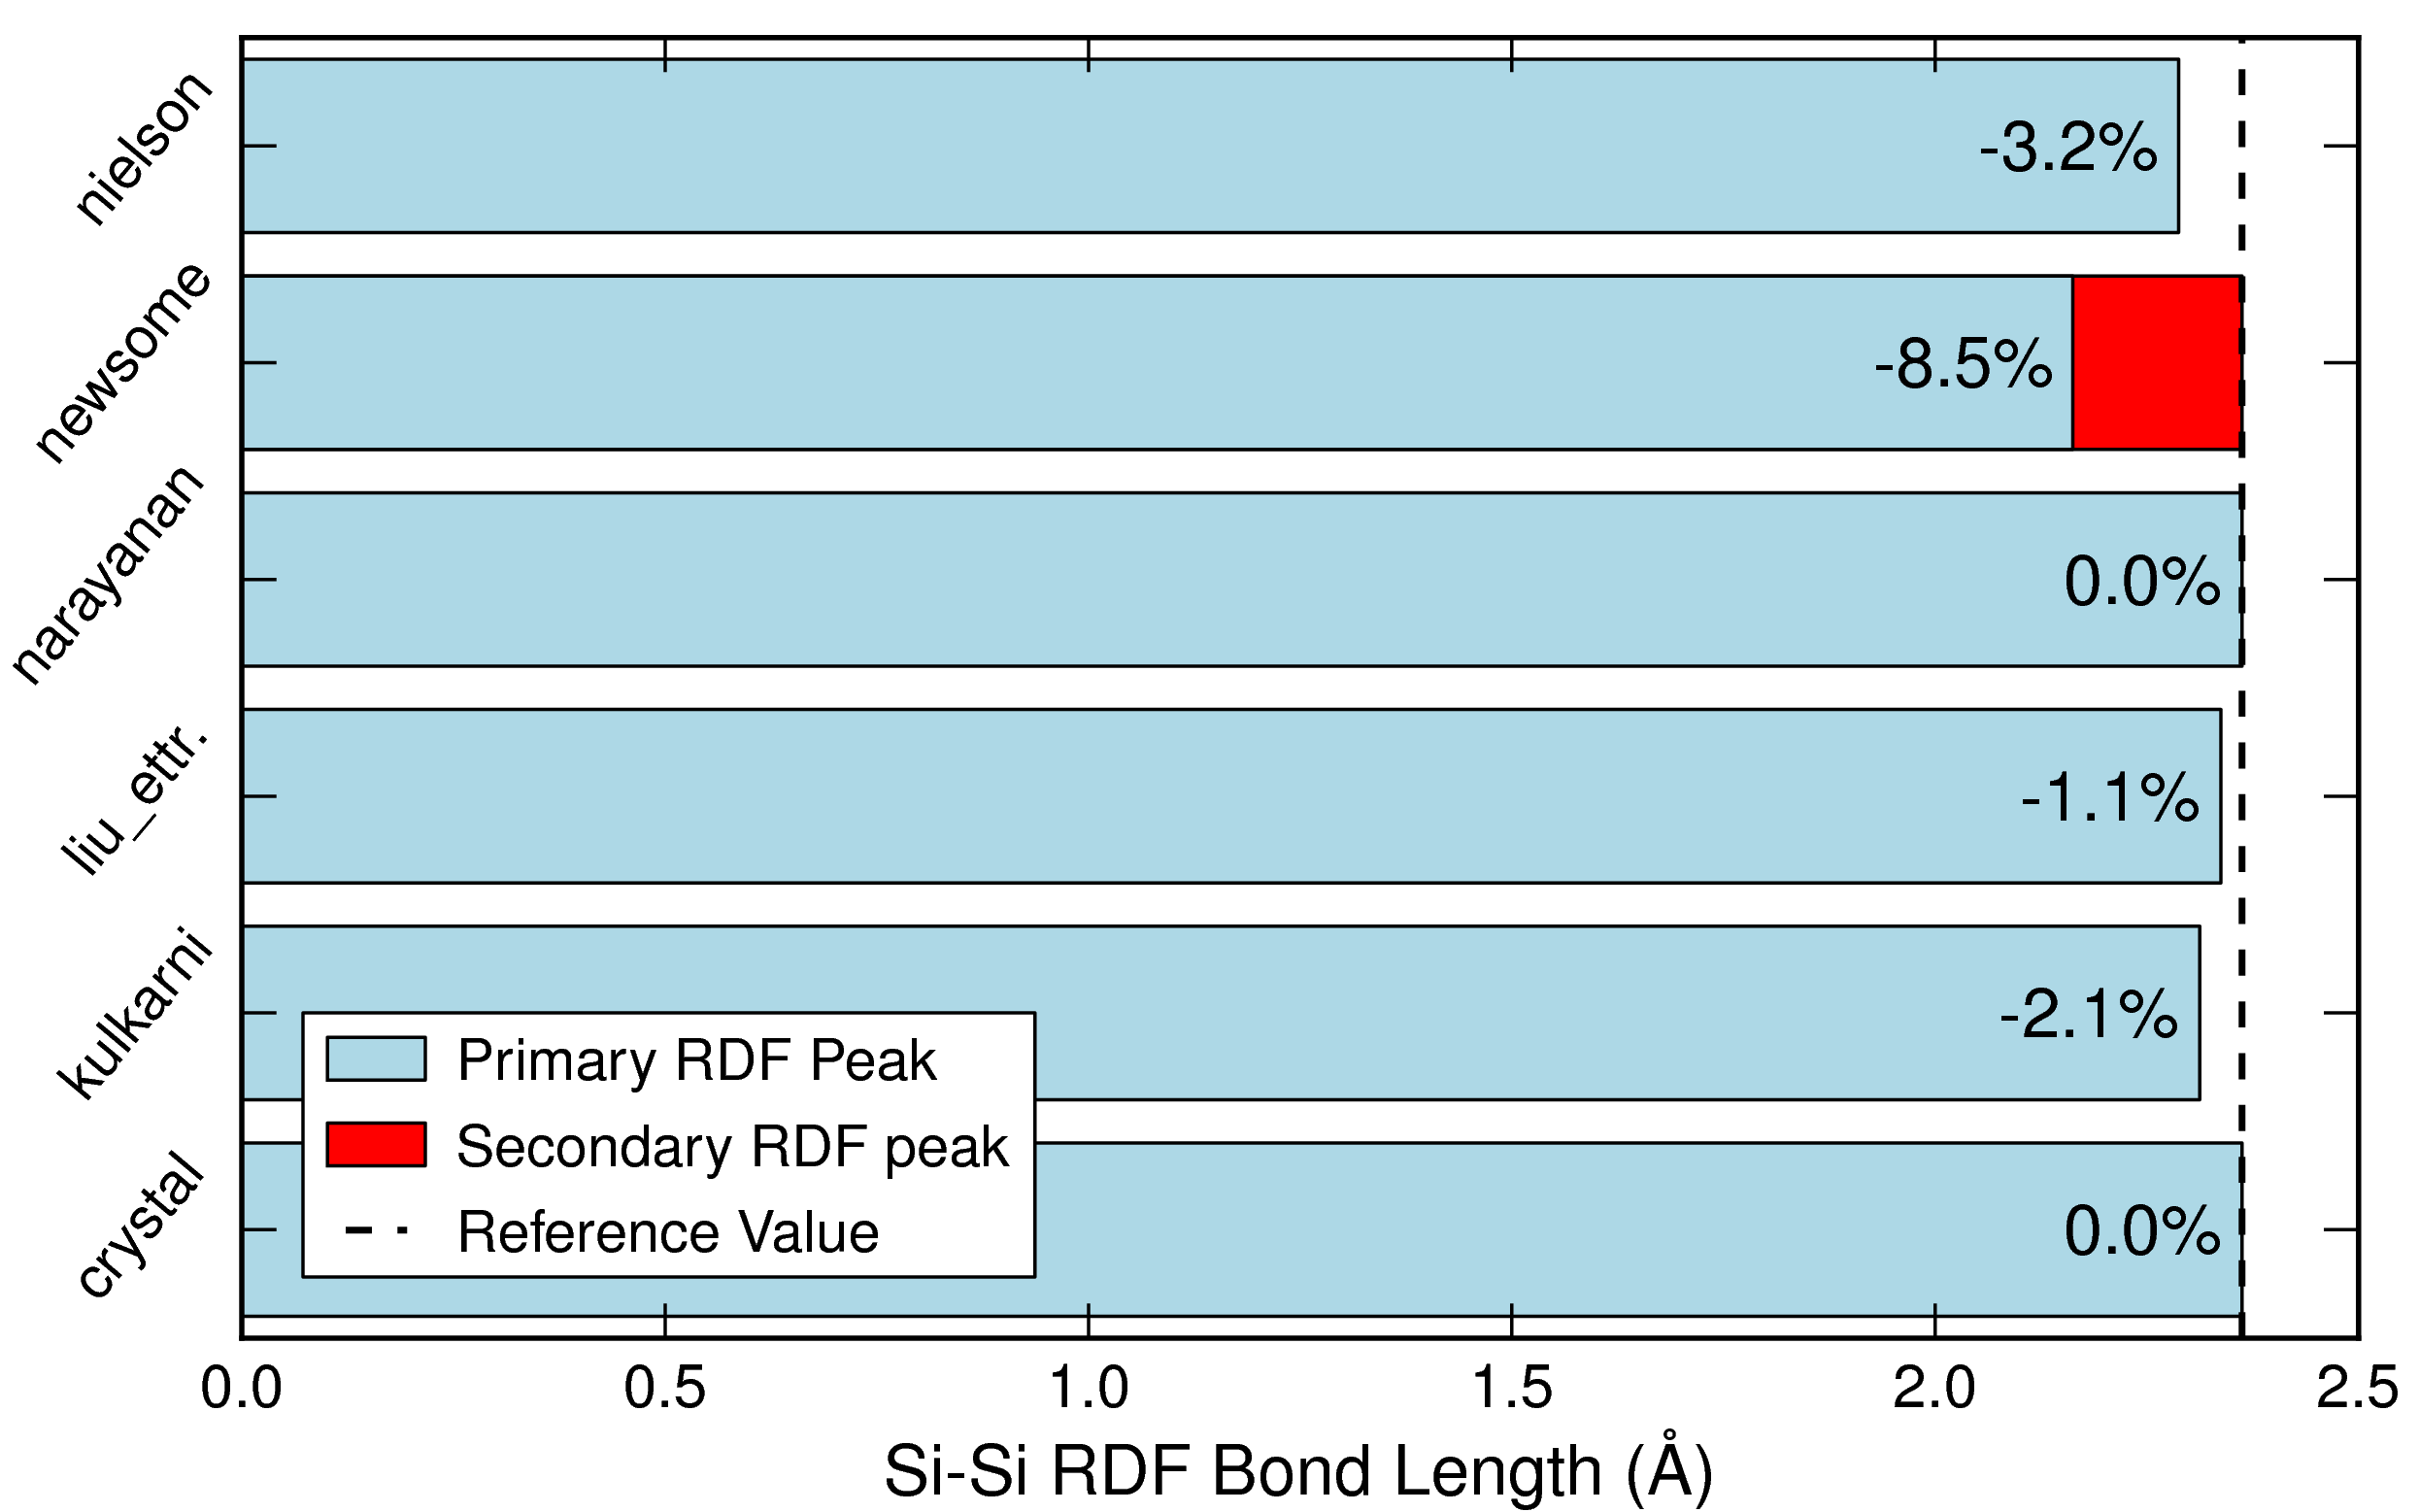
\includegraphics[width=10cm]{SiSi_npt_bondlengths}
  \caption{Bindungslängen von c-\ce{Si} für ReaxFF-Parametrisierungen}
  \label{fig:sisibondlengths}
\end{figure}

Die radialen Verteilungsfunktionen des Kulkarni-Potentiales in Abbildung~\ref{fig:kulkarnirdf} zeigen vollständige Übereinstimmung mit der RDF des Kristalles nach thermischer Relaxierung im kanonischen Ensemble.
Im isotherm-isobaren Ensemble schrumpft der Kristall zwar um \SI{2.1}{\percent}, behält seine Struktur aber ohne weitere Einschränkung bei.
Während der Relaxierung wurde der Kristall auf \SI{500}{\kelvin} erhitzt, wodurch sich die RDF-Spitzen verbreitert und dabei überlagert haben, beim Abkühlen aber wieder zur idealen Kristallstruktur zusammenzogen.

\begin{figure}[!ht]
  \centering
  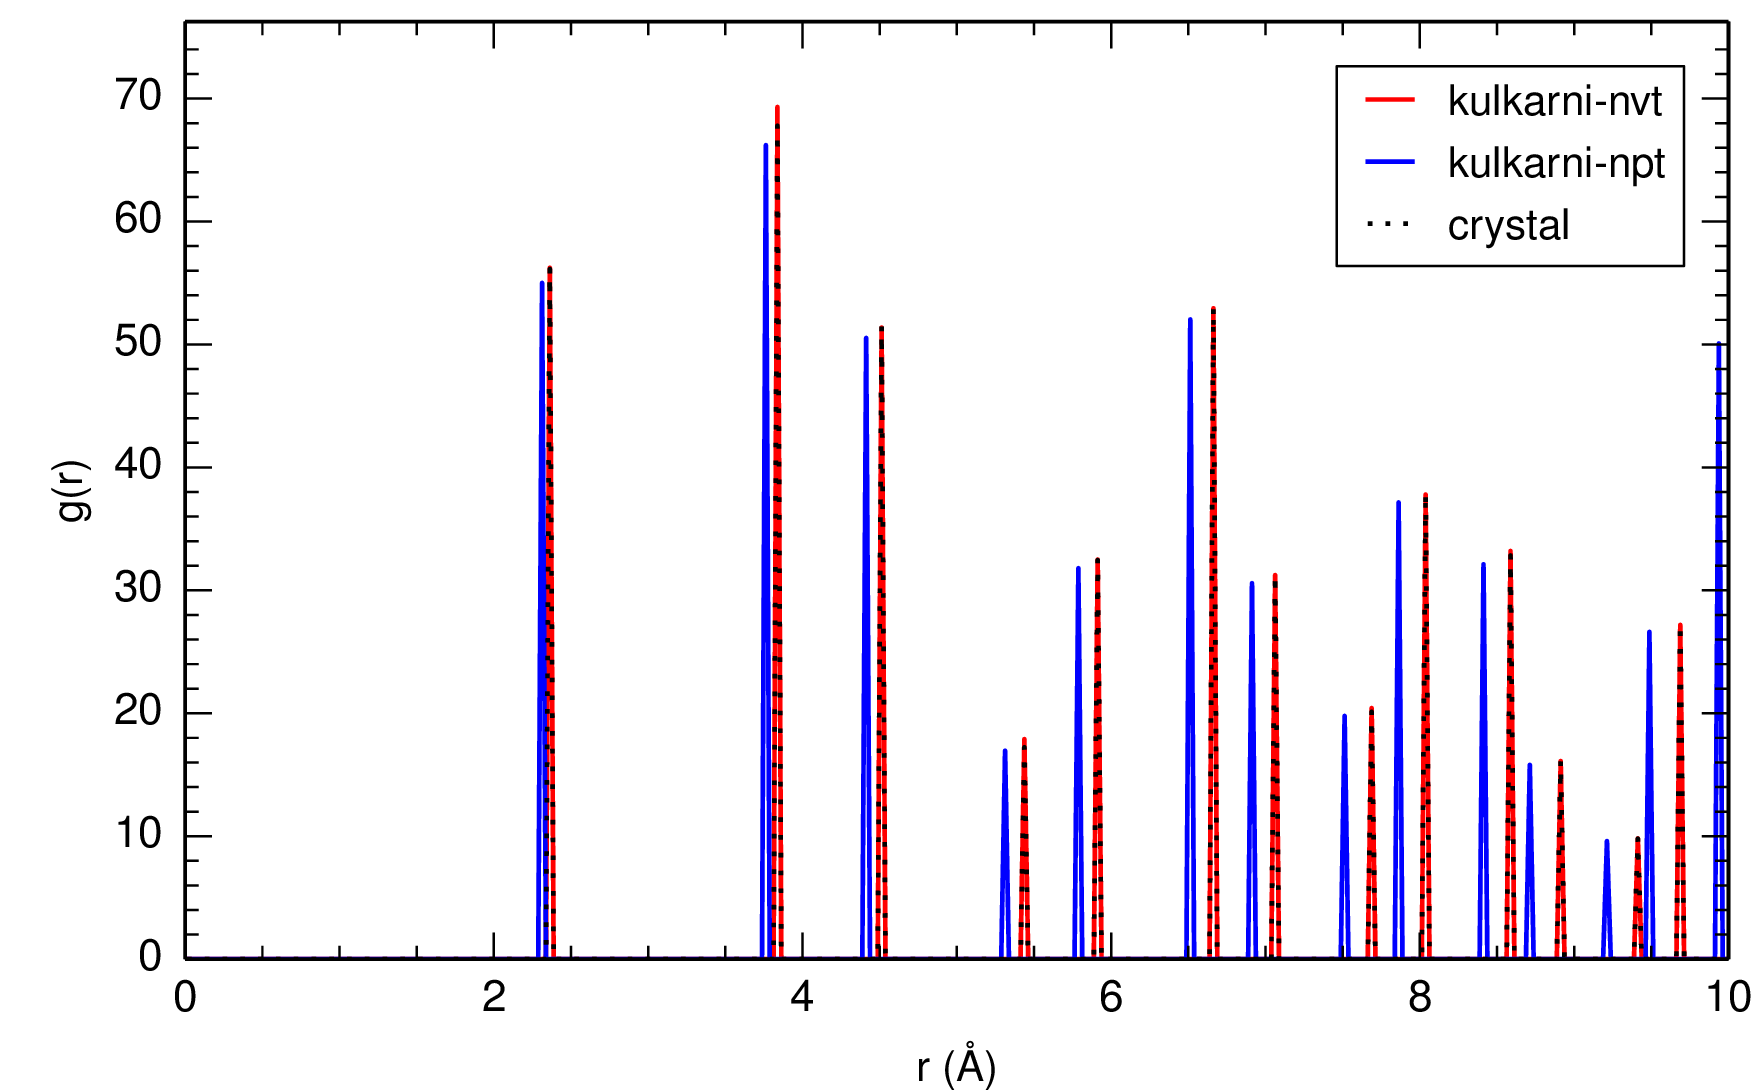
\includegraphics[width=10cm]{kulkarni_rdf_crystal}
  \caption[Radiale Verteilungsfunktionen von relaxiertem c-\ce{Si}]{
    Radiale Verteilungsfunktionen von relaxiertem c-\ce{Si} mit kulkarni
  }
  \label{fig:kulkarnirdf}
\end{figure}

Bei Relaxierung von amorphem Silizium nach den oben beschriebenen Methoden ist anhand der RDF in Abbildung~\ref{fig:amorphousrdf} keine Kristallisation zu erkennen.
Bereits nach \SI{4}{\angstrom} ist keine langreichweitige Ordnung erkennbar, doch ist die Bindungslänge bei \SI{2.339}{\angstrom} klar erkennbar.
Damit liegt sie ca. \SI{3}{\percent} oberhalb ihrer kristallinen Bindungslänge.
Weitere strukturelle Werte für alle untersuchten Parametrisierungen sind in Tabelle~\ref{tab:amorphoussilicon} zu finden.
Der Newsome-Parametersatz generiert eine zusätzliche Spitze in der radialen Verteilungsfunktion vor der eigentlichen Bindungslänge, welche bei amorphen Systemen zu einer Unterschätzung der Bindungslänge und Koordinationszahl führt.

\begin{figure}[!ht]
  \centering
  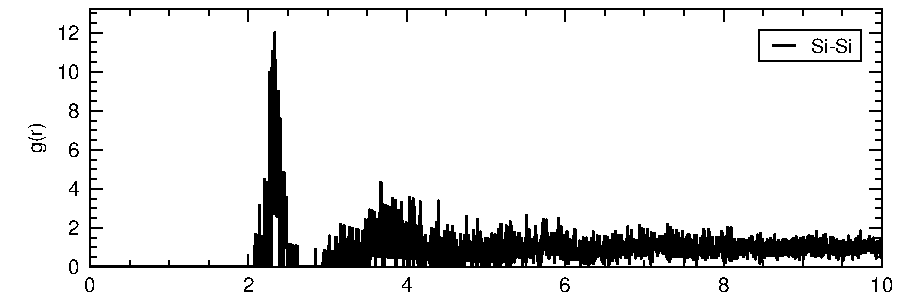
\includegraphics[width=\textwidth]{kulkarni_rdf_amorphous}
  \caption[Radiale Verteilungsfunktionen von relaxiertem a-\ce{Si}]{
    Radiale Verteilungsfunktionen von relaxiertem a-\ce{Si} mit kulkarni
    }
  \label{fig:amorphousrdf}
\end{figure}

\begin{table}[!ht]
  \begin{threeparttable}

    \caption{Vergleich der Struktur amorphen Siliziums}
    \label{tab:amorphoussilicon}

    \oddrowcolors
    \begin{tabularx}{\textwidth}{|llXXlX|}
      \hline
      \textbf{Parametrisierung} & \multicolumn{2}{l}{\textbf{Bindungslänge}}   & \textbf{Koord.} & \textbf{Dichte}    & ~                        \\
      \hline
      (kristallin)              & \SI{2.352}{\angstrom} & ~                    & \num{4.00}      & \SI{2.3296}{\gpcc} & ~                        \\
      amorph                    & ~                     & ~                    & ~               & \SI{2.29}{\gpcc} \cite{remes_optical_1998} &  \\
      \pot{Al\_Al0\_AlN}        & \SI{2.379}{\angstrom} & \SI{+1.15}{\percent} & \num{4.59}      & \SI{2.373}{\gpcc}  & \SI{+3.62}{\percent}     \\
      \pot{kulkarni}            & \SI{2.339}{\angstrom} & \SI{-0.55}{\percent} & \num{4.05}      & \SI{2.361}{\gpcc}  & \SI{+3.10}{\percent}     \\
      \pot{liu\_ettr.}          & \SI{2.401}{\angstrom} & \SI{+2.08}{\percent} & \num{4.10}      & \SI{2.314}{\gpcc}  & \SI{+1.05}{\percent}     \\
      \pot{narayanan}           & \SI{2.383}{\angstrom} & \SI{+1.32}{\percent} & \num{4.05}      & \SI{2.365}{\gpcc}  & \SI{+3.28}{\percent}     \\
      \pot{newsome}             & \SI{2.153}{\angstrom} & \SI{-8.46}{\percent} & \num{1.17}      & \SI{2.398}{\gpcc}  & \SI{+4.72}{\percent}     \\
      \pot{nielson}             & \SI{2.411}{\angstrom} & \SI{+2.51}{\percent} & \num{4.82}      & \SI{2.358}{\gpcc}  & \SI{+2.97}{\percent}     \\
      \pot{zhang}               & \SI{2.357}{\angstrom} & \SI{+0.21}{\percent} & \num{4.39}      & \SI{2.329}{\gpcc}  & \SI{+1.70}{\percent}     \\
      \hline
    \end{tabularx}

  \end{threeparttable}
\end{table}

\section{Struktur der amorphen Schicht nach einer Parsivald-Simulation}

Die Rauheit der aufgewachsenen Schicht hängt stark mit der Bildung und dem Wachstum der Poren zusammen, wodurch das lineare Wachstum der Poren für einen linearen Anstieg der RMS-Rauheit sorgt.
Mit der Schließung der Poren ist eine schlagartige Reduktion der Rauheit zu erwarten, welcher sich gegen Ende der Simulation bereits andeutet, aber nicht mehr statt findet.
Simulationen über längere Zeiträume und größere Schichten sind notwendig, diesen Effekt näher zu charakterisieren

\begin{figure}[ht]
  \centering
  \captionsetup[subfigure]{singlelinecheck=false}
  \def\subfigwidth{0.48\textwidth}
  \begin{subfigure}[t]{\subfigwidth}
    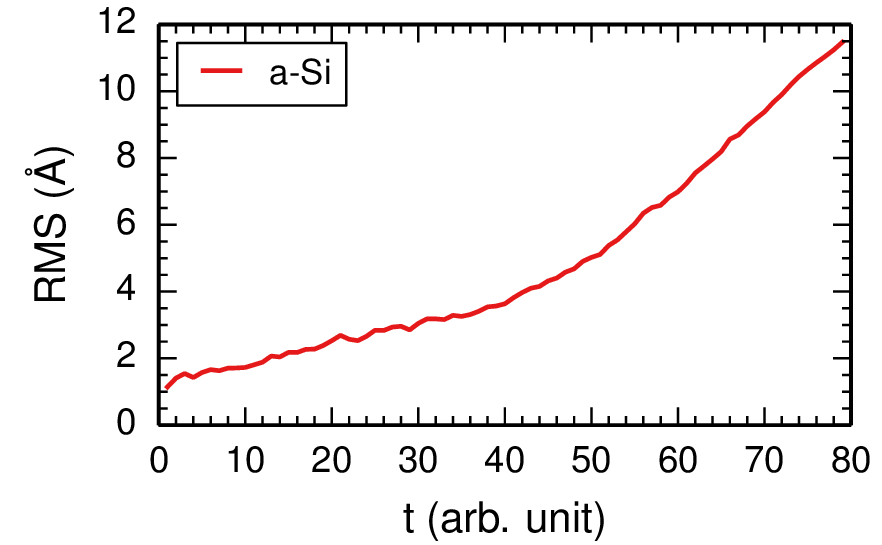
\includegraphics[width=\textwidth]{Si111_roughness}
    %% \subcaption{Dicke und Rauheit der Schicht}
    %% \label{fig:siliconresults-a}
  \end{subfigure}
  \caption{Zeitliche Entwicklung der Rauheit einer Silizium-PVD-Schicht}
  \label{fig:siliconroughness}
\end{figure}

\section{Precursorsimulationen}

ReaxFF-Potentiale versprechen die Simulation von Molekülen und deren Reaktion miteinander, die mit den folgenden Tests für Silan und molekularen Sauerstoff überprüft werden sollen.

\subsection{Stabilität der Precursormoleküle (\ce{SiH4}, \ce{O2})}

Simulationen einzelner und mehrerer Precursormoleküle (\ce{SiH4} und \ce{O2}) hinsichtlich ihrer Stabilität wurden im mikrokanonischen beziehungsweise kanonischen Ensemble bei verschiedenen Temperaturen durchgeführt.
\todo{Abbildung hier her kopieren}Abbildung~\ref{fig:silanestability} zeigt eine Auswahl der Ergebnisse der Silan-Simulationen, an denen sich erkennen lässt, wie instabile Simulationen zur Ablösung der Wasserstoffatome vom Silanmolekül führen.

\todoline{Joerg: Letztlich benutzt du doch den Strukturgenerator, der die atomare Struktur einer Vielzahl von relevanten Materialien in ihrer jeweils idealen Kristallstruktur generiert. Dabei wird doch auf tabellierte Werte der Bindungslängen zurück gegriffen.}
\todoline{Für Moleküle vereinfacht sich das auf Standard-Bindungslängen und Standard-Bindungswinkel, die man Wo findet? -> CRC?!?}
Zur Simulation der Stabilität von Silan wurde dieses mit \todo{vorstellen, woher die Werte kommen und warum das eine ordentliche Struktur ist}Materials Studio präpariert und anschließend im mikrokanonischen Ensemble mit einer anfänglichen Temperatur von \SIrange{300}{700}{\kelvin} relaxiert.
Eine Strukturoptimierung wurde nicht durchgeführt, da die thermische Stabilität untersucht werden sollte und die untersuchten Moleküle keine komplizierten Strukturen beinhalten.

Bei Al\_Al0\_AlN, Kulkarni, Nielson und Zhang behalten die Silan-Moleküle ihre Struktur, während die einige der \ce{Si-H}-Bindungen bei den anderen Parametrisierungen brechen und einzelne Wasserstoff-Moleküle freigeben (Abbildung~\ref{fig:silanestability}).
Dieser Effekt ist unabhängig von der anfänglichen Temperatur.

\begin{figure}[!ht]

  \captionsetup[subfigure]{singlelinecheck=false}
  \def\subfigwidth{0.32\textwidth}
  \begin{subfigure}[t]{3.5cm}
    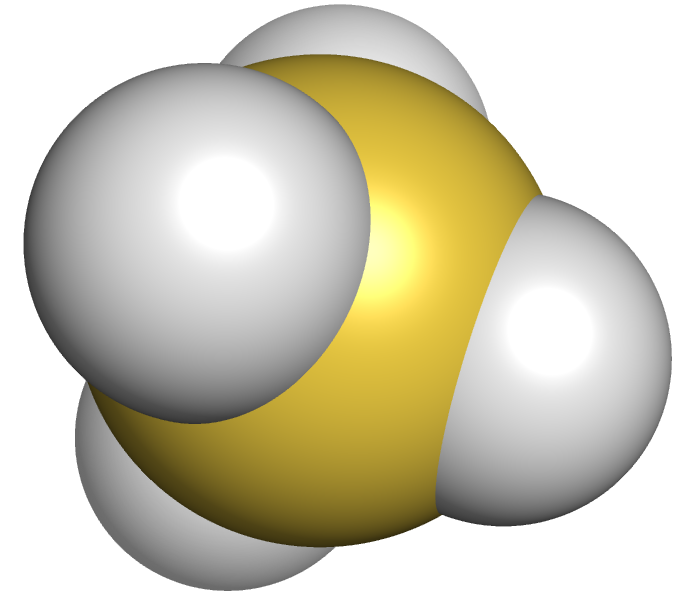
\includegraphics[width=\textwidth]{silane_nielson_stable}
    \subcaption{nielson: stabil}
  \end{subfigure}
  \hfill
  \begin{subfigure}[t]{4.5cm}
    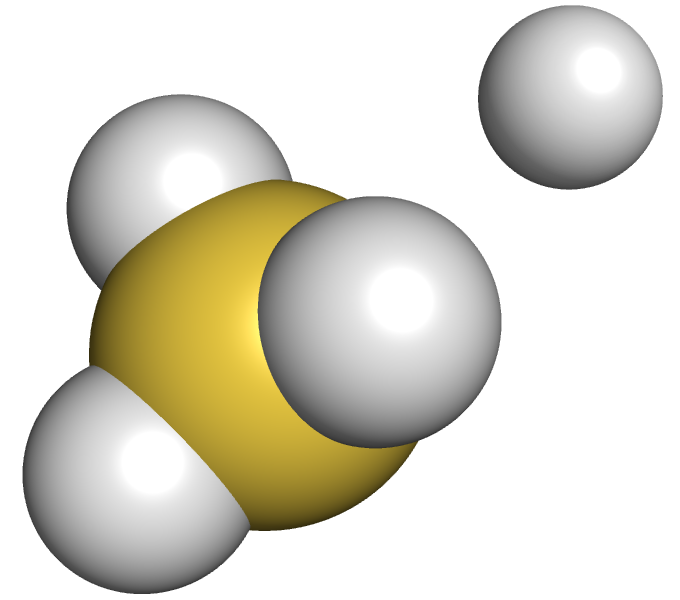
\includegraphics[width=\textwidth]{silane_narayanan_unstable}
    \subcaption{narayanan: instabil}
  \end{subfigure}
  \hfill
  \begin{subfigure}[t]{5cm}
    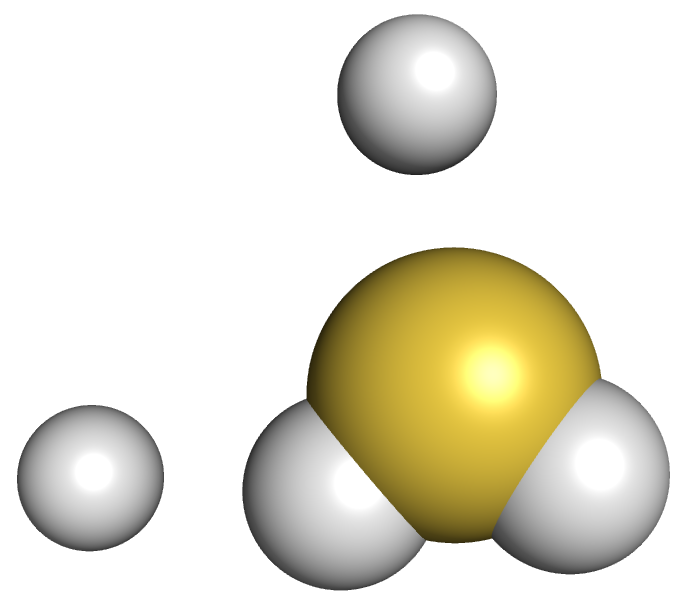
\includegraphics[width=\textwidth]{silane_liu_unstable}
    \subcaption{liu-ettringite: instabil}
  \end{subfigure}

  \caption[Stabilitätsuntersuchungen von Silan]{
    Stabilitätsuntersuchungen von Silan (\ce{SiH4}) bei 600K (CVD-Temperatur)
  }
  \label{fig:silanestability}

\end{figure}

\subsection{Reaktion der Precursormoleküle (\ce{SiH4 + O2})}

Reaktionen von einzelnen Precursormolekülen wurden stichprobenartig in verschiedenen Orientierungen, Energien und Temperaturen vorgenommen, um einen Überblick über die Verlässlichkeit zu bekommen.
Zusätzlich wurden durchmischte Precursorgase mit dem Ziel eventueller Reaktionen simuliert, was jedoch mit keiner der Parametrisierungen zum gewünschten Erfolg bei hoher Zuverlässigkeit führte.
Einige Parametrisierungen zeigen jedoch vielversprechende Teilreaktionen, die korrekte Doppelbindungen und Bildung von Wasserstoffmolekülen beinhalten (Abbildung~\ref{fig:precursorreactions}).
Vor allem bei größeren Simulationsräumen bilden sich Cluster aus Precursormolekülen, die von attraktiven Termen in den Kraftfeldern dominiert werden, aber nicht durch chemische Wechselwirkungen zu erklären sind (Abbildung~\ref{fig:precursorclusters}).

Für die Reaktion von Silan mit Wasser wurden beide Moleküle außerhalb der Cutoff-Reich\-weite der ReaxFF-Potentiale (in der Regel \SI{6}{\angstrom}) mit zufälligen Orientierungen platziert und zusätzlich zu einer geringen Anfangsgeschwindigkeit zueinander beschleunigt.
Die relativen kinetischen Energien reichen von \SI{0.1}{\electronvolt} bis \SI{10}{\electronvolt} und decken somit einen breiten Geschwindigkeitsbereich ab.

Die meisten Parametrisierungen zeigen keine Änderung des Bindungszustandes der Moleküle, allerdings zeigen Zhang, Newsome und Kulkarni bindendes Verhalten (Abbildung~\ref{fig:precursorreactions}).
Einige der Zhang-Simulationen zeigen, wie in der Abbildung dargestellt, eine Überzahl an stabilen Bindungen, doch lösen sich diese bei höheren Anfangsgeschwindigkeiten.
Die beiden anderen Potentiale zeigen meist die korrekte Zahl an Bindungen für das Silizium-Atom, doch bildet sich meist atomarer Sauer- und Wasserstoff, der allerdings bei Kontakt mit einem anderen Atom Bindungen aufbauen müsste.

Bei der Reaktion mehrer Precursor-Moleküle im kanonischen Ensemble zeigen sich gravierendere Unterschiede (Abbildung~\ref{fig:precursorclusters}).
Kulkarni-Simulationen bilden etwa Sauerstoff-Cluster sowie Bindungen zwischen den Wasserstoff-Atomen der Silan-Moleküle.
Einzig Zhang stellt teilweise korrekte Bindungen dar, was vermutlich durch die Anwendung zur Beschreibung von Reaktionen vergleichsweise großer Moleküle gegeben ist.
Es zeigen sich jedoch auch hier Überkoordinationen, wie sie bereits in Abbildung~\ref{fig:precursorreactions} beobachtet werden konnten.
Eine Simulation mit Newsome wurde aufgrund der instabilen Silan-Moleküle nicht durchgeführt.

\begin{figure}[!ht]

  \captionsetup[subfigure]{singlelinecheck=false}
  \def\subfigwidth{0.32\textwidth}
  \begin{subfigure}[t]{3cm}
    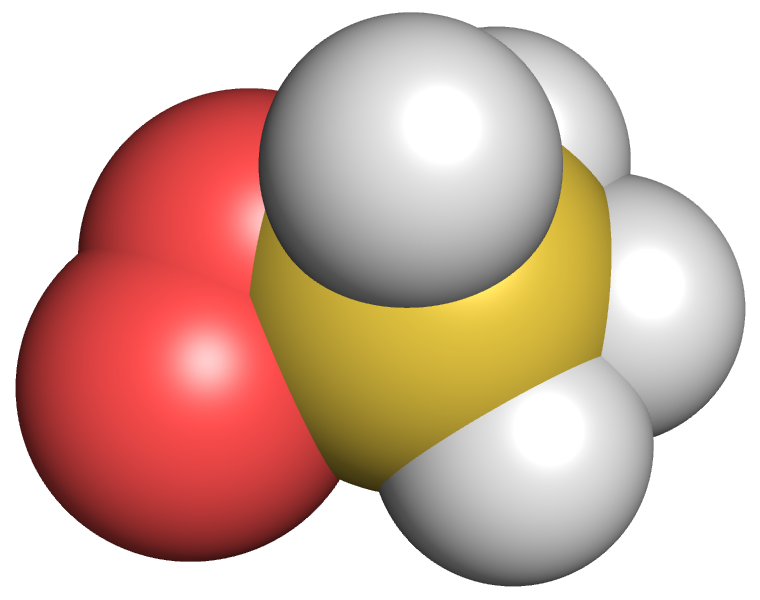
\includegraphics[width=\textwidth]{silane_reaction_zhang}
    \subcaption{zhang: Überzahl an Bindungen}
  \end{subfigure}
  \hfill
  \begin{subfigure}[t]{5cm}
    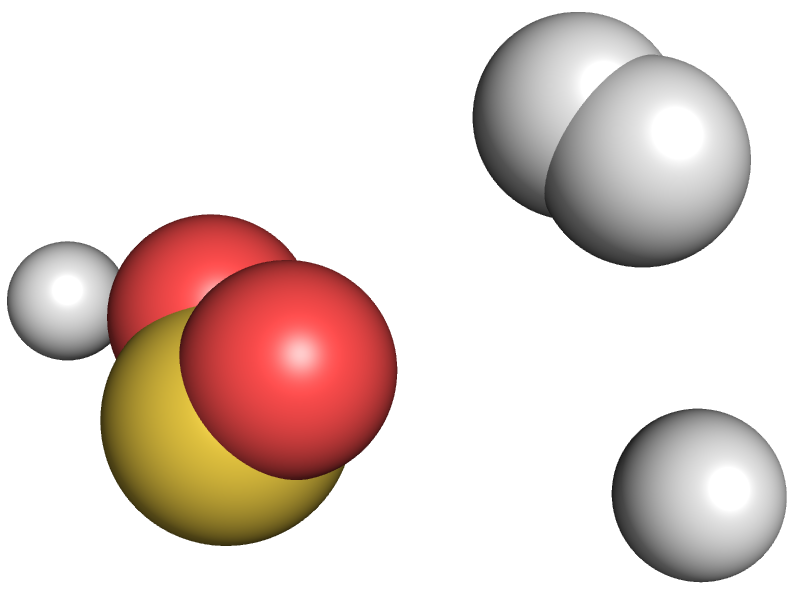
\includegraphics[width=\textwidth]{silane_reaction_newsome}
    \subcaption{newsome: korrekte Stöchiometrie}
  \end{subfigure}
  \hfill
  \begin{subfigure}[t]{4.5cm}
    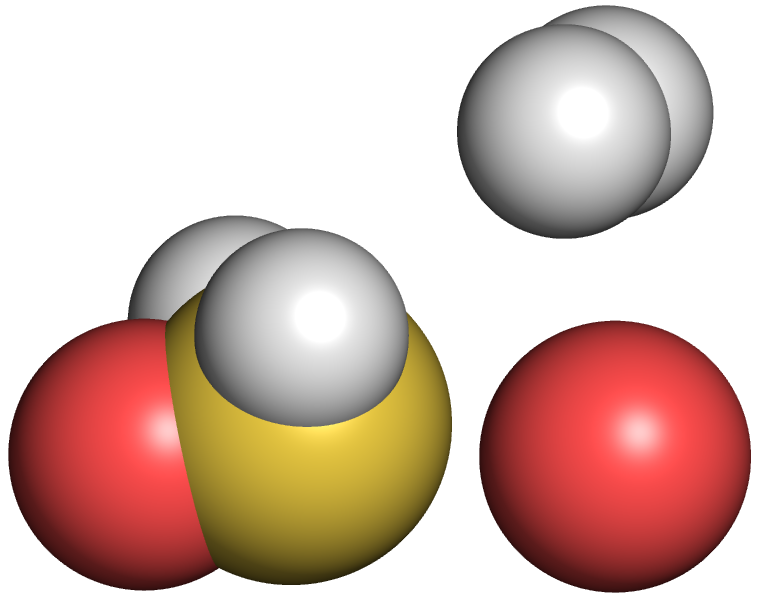
\includegraphics[width=\textwidth]{silane_reaction_kulkarni}
    \subcaption{kulkarni: Korrekte \ce{Si}-Bindungen, aber \ce{O}-Atom}
  \end{subfigure}

  \caption[Reaktionen von \ce{SiH4} mit \ce{O2}]{
    Reaktion von \ce{SiH4} mit \ce{O2}
  }
  \label{fig:precursorreactions}

\end{figure}

\begin{figure}[!ht]

  \captionsetup[subfigure]{singlelinecheck=false}
  \begin{subfigure}[t]{4cm}
    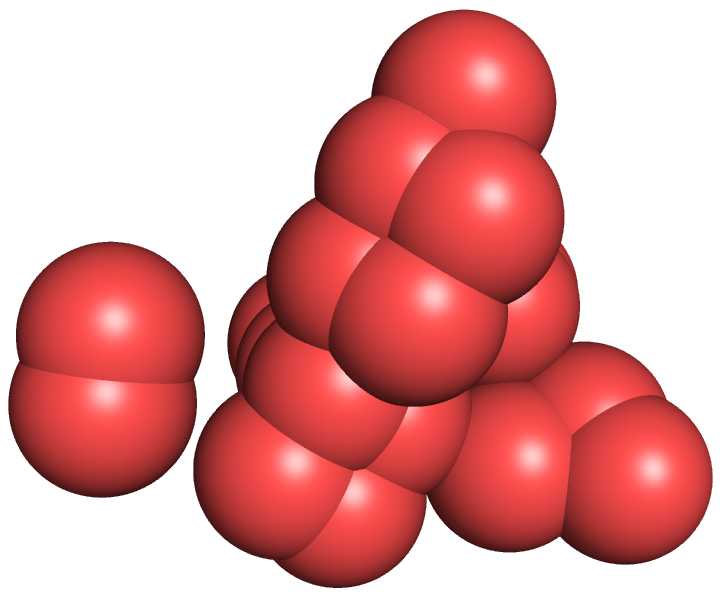
\includegraphics[width=\textwidth]{oxygen_cluster}
    \subcaption{kulkarni: \ce{O2}-Cluster}
  \end{subfigure}
  \hfill
  \begin{subfigure}[t]{5.5cm}
    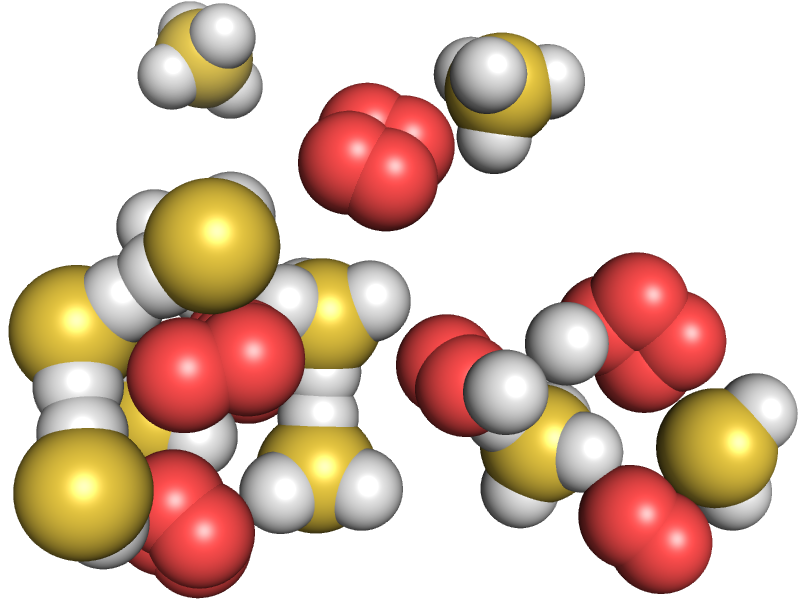
\includegraphics[width=\textwidth]{kulkarni_precursor_cluster}
    \subcaption{kulkarni: Precursor-Cluster}
  \end{subfigure}
  \hfill
  \begin{subfigure}[t]{4.5cm}
    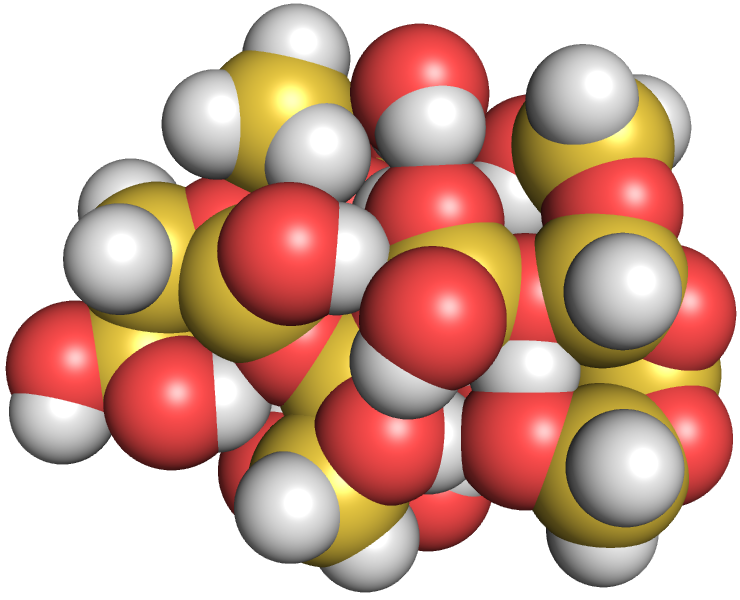
\includegraphics[width=\textwidth]{zhang_precursor_cluster}
    \subcaption{zhang: Reaktionen}
  \end{subfigure}

  \caption[Cluster von Precursormolekülen]{Clusterbildung und partielle Reaktionen von Precursormolekülen bei 500K}
  \label{fig:precursorclusters}

\end{figure}
